\subsubsection{usergoal-ugGlobalDispatchManagement}

\label{RE-use-case-ugGlobalDispatchManagement}


Shows the ugGlobalDispatchManagement use-case and its actors.		  


\begin{usecase}
  \addheading{Use-Case Description}
  \addsingletwocolumnrow{Name}{ugGlobalDispatchManagement}
  \addsingletwocolumnrow{Scope}{system}
  \addsingletwocolumnrow{Level}{usergoal}
  

\addrowheading{Primary actor(s)}
\addnumberedsinglerow{}{\msrcode{actFiremenCoordinator[active]}}


\addrowheading{Secondary actor(s)}
\addnumberedsinglerow{}{\msrcode{actCentralCoordinator[active]}}
\addnumberedsinglerow{}{\msrcode{actTowServiceCoordinator[active]}}
\addnumberedsinglerow{}{\msrcode{actPoliceCoordinator[active]}}

\addrowheading{Goal(s) description}
\addsinglerow{Shows the ugGlobalDispatchManagement use-case and its actors.}


\addrowheading{Protocol condition(s)}
\addnumberedsinglerow{}{
}

\addrowheading{Pre-condition(s)}
\addnumberedsinglerow{}{
}

\addrowheading{Main post-condition(s)}
\addnumberedsinglerow{}{
}

\addrowheading{Main Steps}
\addalphanumberedsinglerow{}{the actor \msrcode{actFiremenCoordinator} executes the \msrucname{oeUpdateDispatchStatus} use case}
\addalphanumberedsinglerow{}{the actor \msrcode{actTowServiceCoordinator} executes the \msrucname{oeRefreshMap} use case}
\addalphanumberedsinglerow{}{the actor \msrcode{actTowServiceCoordinator} executes the \msrucname{oeMessage} use case}
\addalphanumberedsinglerow{}{the actor \msrcode{actTowServiceCoordinator} executes the \msrucname{oeUpdateDispatchStatus} use case}
\addalphanumberedsinglerow{}{the actor \msrcode{actFiremenCoordinator} executes the \msrucname{oeRequestHelp} use case}
\addalphanumberedsinglerow{}{the actor \msrcode{actPoliceCoordinator} executes the \msrucname{oeUpdateDispatchStatus} use case}
\addrowheading{Steps Ordering Constraints}
\addnumberedsinglerow{}{step (a) must be executed at least two times}
\addnumberedsinglerow{}{step (d) must be executed at least two times}
\addnumberedsinglerow{}{step (f) can only be executed if step (e) has at least been executed once previously}
\addnumberedsinglerow{}{step (f) must be executed at least two times}

\addrowheading{Additional Information}
\addsinglerow{
none
}

\end{usecase} 


Figure \ref{fig:lu.uni.lassy.excalibur.group09.spec-RE-UCD-uc-ugGlobalDispatchManagement}
Shows the ugGlobalDispatchManagement use-case and its actors.

\begin{figure}[htbp]
\begin{center}

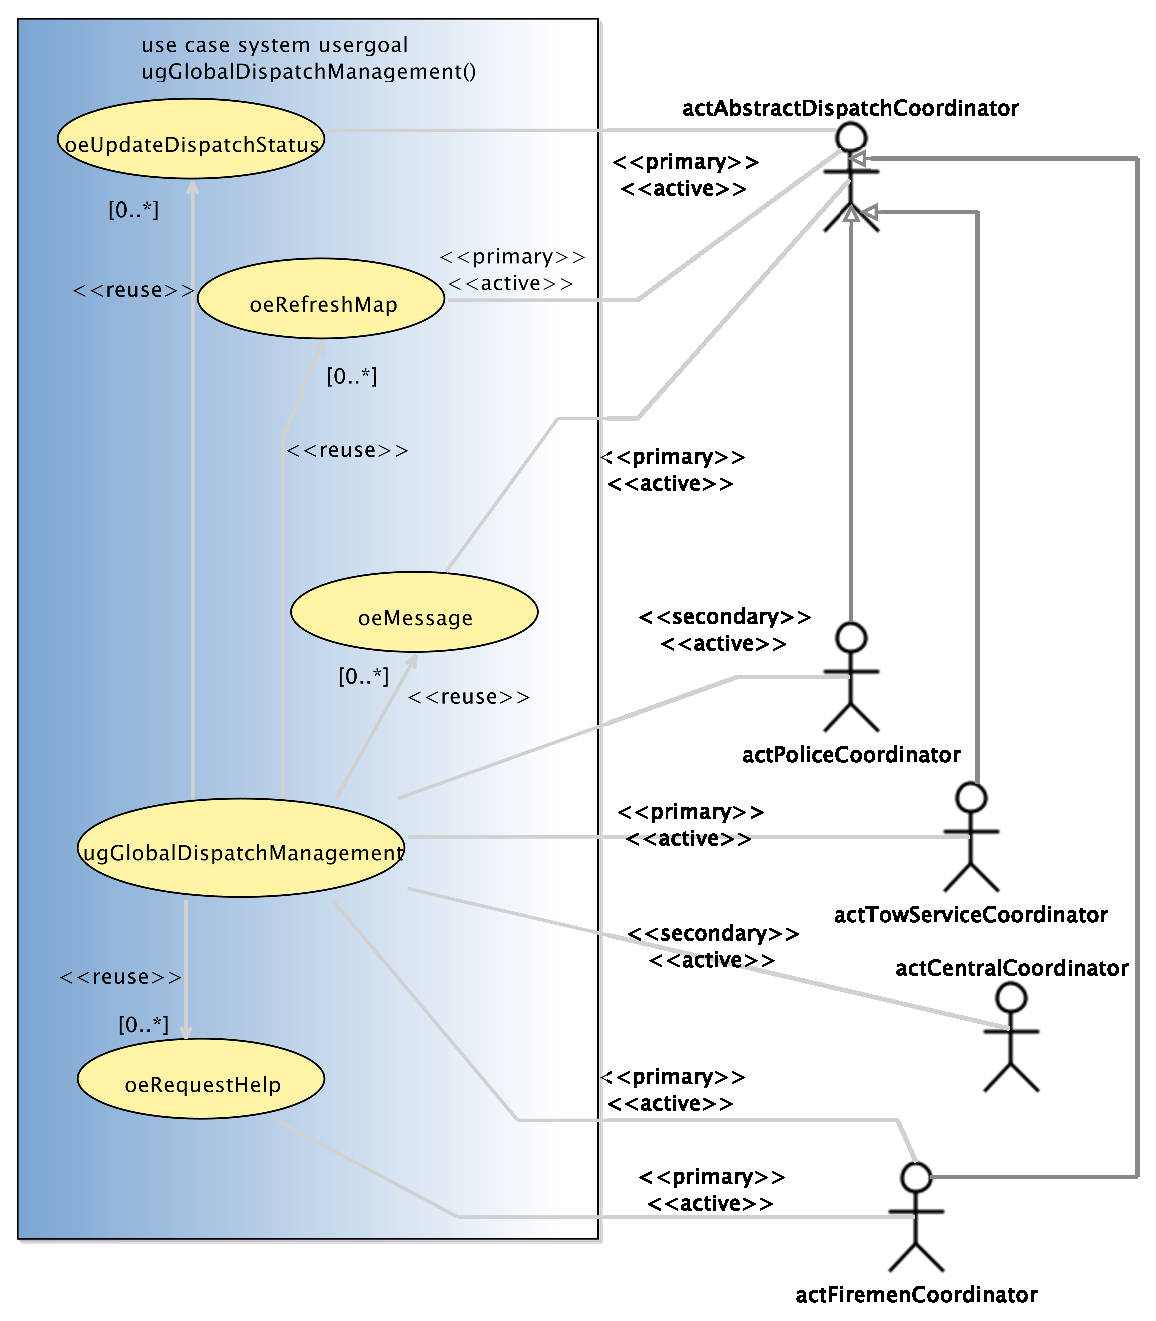
\includegraphics[
angle=0
,width=1.0\textwidth
]{./images-report-gen/usecase-model/usergoal/uc-ugGlobalDispatchManagement.eps}
\end{center}
\caption[lu.uni.lassy.excalibur.group09.spec Use Case Diagram: uc-ugGlobalDispatchManagement]{}
\label{fig:lu.uni.lassy.excalibur.group09.spec-RE-UCD-uc-ugGlobalDispatchManagement}
\end{figure}
\vspace{0.5cm}
